\section{L-BFGS}
\label{sec:qn-lbfgs}

BFGS不必解方程，但仍要保存一个$n\times n$的稠密矩阵。$n=10^6$时这需要约$10^{12}$个元素的存储，通常根本放不下。不保存矩阵，能否仍然算出$\bm{W}^{(t)}\bm{g}^{(t)}$？

\paragraph{主要思想：只保留最近的测量}
BFGS的$\bm{W}^{(t)}$完全由$\bm{W}^{(0)}$和所有的$(\bm{s}^{(j)},\bm{y}^{(j)})$决定。旧测量在非二次目标上已经过时，于是\term{有限记忆BFGS}（limited-memory BFGS，L-BFGS）只保留最近$r$对，$r$称为记忆长度，常取$3$到$30$。

存储从约$n^2/2$个数降到$2rn$个数。每一轮都重新从一个简单的初始矩阵$\gamma^{(t)}\bm{I}$出发，把这$r$对依次用式~\eqref{eq:qn-bfgs-inverse}更新一遍，得到的矩阵就是这一轮的$\bm{W}^{(t)}$。

记下面$r$次更新的中间矩阵为$\bm{W}_{[j]}$，下标$j$从$t-r$走到$t$。起点和递推是
\begin{equation}
 \bm{W}_{[t-r]}=\gamma^{(t)}\bm{I},\qquad
 \bm{W}_{[j+1]}=\bigl(\bm{V}^{(j)}\bigr)^\top\bm{W}_{[j]}\bm{V}^{(j)}+\rho^{(j)}\bm{s}^{(j)}\bigl(\bm{s}^{(j)}\bigr)^\top,
 \label{eq:qn-lbfgs-recursion}
\end{equation}
其中$\bm{V}^{(j)}$由第$j$对向量按定理~\ref{thm:qn-bfgs-inverse}的方式构成，最后$\bm{W}^{(t)}=\bm{W}_{[t]}$。显式写出这些矩阵要$O(n^2)$的存储，我们其实只需要它乘一个向量的结果。

\paragraph{主要思想：两层递推}
令$\bm{q}_{[t]}=\bm{g}^{(t)}$，想算$\bm{W}_{[t]}\bm{q}_{[t]}$。把递推~\eqref{eq:qn-lbfgs-recursion}作用在向量$\bm{q}_{[j+1]}$上，先算出向右侧的两个量：
\[
 \xi^{(j)}=\rho^{(j)}\langle\bm{s}^{(j)},\bm{q}_{[j+1]}\rangle,\qquad
 \bm{q}_{[j]}=\bm{V}^{(j)}\bm{q}_{[j+1]}=\bm{q}_{[j+1]}-\xi^{(j)}\bm{y}^{(j)}.
\]

于是一次更新对向量的作用可以写成
\[
 \bm{W}_{[j+1]}\bm{q}_{[j+1]}=\bigl(\bm{V}^{(j)}\bigr)^\top\bm{W}_{[j]}\bm{q}_{[j]}+\xi^{(j)}\bm{s}^{(j)}.
\]
右端的$\bm{W}_{[j]}\bm{q}_{[j]}$是同样形式、但下标小一的问题。所以计算分两层：第一层让$j$从$t-1$递减到$t-r$，把$\bm{q}$一路算下去，记下所有$\xi^{(j)}$。

第一层走到底时，最内层的矩阵是$\gamma^{(t)}\bm{I}$，令$\bm{z}_{[t-r]}=\gamma^{(t)}\bm{q}_{[t-r]}$。记$\bm{z}_{[j]}=\bm{W}_{[j]}\bm{q}_{[j]}$，把$\bm{V}^{(j)}$的转置展开，得到第二层的递推：
\begin{equation}
 \eta^{(j)}=\rho^{(j)}\langle\bm{y}^{(j)},\bm{z}_{[j]}\rangle,\qquad
 \bm{z}_{[j+1]}=\bm{z}_{[j]}+\bigl(\xi^{(j)}-\eta^{(j)}\bigr)\bm{s}^{(j)}.
 \label{eq:qn-lbfgs-second-loop}
\end{equation}
第二层让$j$从$t-r$递增到$t-1$，最后的$\bm{z}_{[t]}$就是$\bm{W}^{(t)}\bm{g}^{(t)}$。这就是\term{双循环递推}（two-loop recursion），图~\ref{fig:qn-lbfgs-two-loop}是它的结构。

\begin{BookInlineFigure}
  \centering
  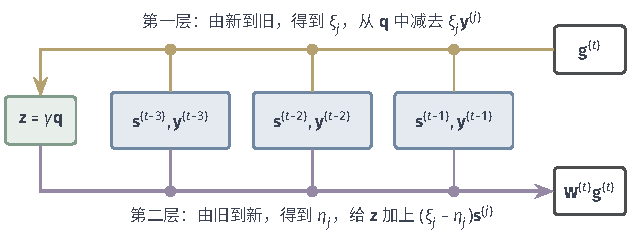
\includegraphics[width=106mm]{figures/05-optimization/02-smooth-optimization/tikz/qn-lbfgs-two-loop/figure.pdf}
  \caption{L-BFGS的双循环递推，$r=3$。蓝框是保存的三对向量。第一层（黄）从梯度出发，由最新一对走到最旧一对；中间乘初始矩阵$\gamma\bm{I}$（绿框）；第二层（紫）由最旧一对走回最新一对，输出$\bm{W}^{(t)}\bm{g}^{(t)}$。全程只有向量内积和向量加法。}
  \label{fig:qn-lbfgs-two-loop}
\end{BookInlineFigure}

每一层对每对向量做一次内积和一次向量加法，再加上中间的缩放，每个方向的运算量约为$(4r+1)n$次乘法。矩阵本身从未出现。

\paragraph{主要思想：初始缩放}
最内层的矩阵决定了双循环不了解的那些方向上的尺度。L-BFGS一般取
\begin{equation}
 \gamma^{(t)}=\frac{\langle\bm{s}^{(t-1)},\bm{y}^{(t-1)}\rangle}{\langle\bm{y}^{(t-1)},\bm{y}^{(t-1)}\rangle}.
 \label{eq:qn-lbfgs-gamma}
\end{equation}

它的含义可以由式~\eqref{eq:qn-average-hessian}看出。设平均Hessian正定，并把$(\bar{\bm{H}}^{(t-1)})^{1/2}\bm{s}^{(t-1)}$记作$\bm{z}$，则
\[
 \frac{1}{\gamma^{(t)}}=\frac{\bm{z}^\top\bar{\bm{H}}^{(t-1)}\bm{z}}{\bm{z}^\top\bm{z}}.
\]
所以$1/\gamma^{(t)}$是平均Hessian的一个Rayleigh商，落在其最小与最大特征值之间，是目标曲率的一个合理的标量估计。

\paragraph{主要思想：曲率检查}
与完整BFGS一样，存入的$(\bm{s}^{(j)},\bm{y}^{(j)})$必须满足$\langle\bm{s}^{(j)},\bm{y}^{(j)}\rangle>0$，否则式~\eqref{eq:qn-lbfgs-recursion}不再保证正定，算出的方向可能不下降。Wolfe线搜索使这一点自动成立。只用回溯时，要加上跳过规则：满足式~\eqref{eq:qn-skip-rule}的这一对不存入，窗口保持原样。

\paragraph{计算过程}
下面用贯穿例演示$r=2$的L-BFGS。为了不让第一层的系数因为正交性而消失，第一步取$\alpha^{(0)}=1/8$而不是精确步长，以后都用单位步长；这些步长都满足$c_1=10^{-4}$、$c_2=0.9$的Wolfe条件。

\needspace{6\baselineskip}
\paragraph{变量}
\begin{itemize}
 \item $\bm{x}^{(t)}$、$\bm{g}^{(t)}\in\mathbb{R}^{n}$：当前点与梯度。
 \item 窗口：最多$r$组$(\bm{s}^{(j)},\bm{y}^{(j)},\rho^{(j)})$，$\bm{s}^{(j)},\bm{y}^{(j)}\in\mathbb{R}^{n}$，$\rho^{(j)}$是标量，从旧到新排列。
 \item 第一层的向量$\bm{q}\in\mathbb{R}^{n}$和系数$\xi^{(j)}$；第二层的向量$\bm{z}\in\mathbb{R}^{n}$和系数$\eta^{(j)}$。
 \item $\gamma^{(t)}>0$：初始矩阵的缩放。
\end{itemize}

\paragraph{初始化}
选起点，窗口置空。窗口为空时取$\gamma^{(0)}=1$，方向就是负梯度。例中第一轮的数据是
\[
 \bm{x}^{(0)}=(4,1)^\top,\qquad\bm{g}^{(0)}=(8,8)^\top,\qquad\bm{d}^{(0)}=(-8,-8)^\top.
\]
取$\alpha^{(0)}=1/8$，走完后有
\[
 \bm{x}^{(1)}=(3,0)^\top,\qquad\bm{g}^{(1)}=(6,0)^\top.
\]
第一对测量及其$\rho$是
\[
 \bm{s}^{(0)}=(-1,-1)^\top,\qquad\bm{y}^{(0)}=(-2,-8)^\top,\qquad\rho^{(0)}=0.1.
\]

\paragraph{每轮更新}
对$t=1,2,\ldots$依次执行下面的步骤，当$\lVert\bm{g}^{(t)}\rVert_2\leq\varepsilon$时停止。

\begin{enumerate}
\item 第一层，令$\bm{q}=\bm{g}^{(t)}$，对窗口中的$j$由新到旧，依次计算
\[
 \xi^{(j)}=\rho^{(j)}\langle\bm{s}^{(j)},\bm{q}\rangle,\qquad\bm{q}\leftarrow\bm{q}-\xi^{(j)}\bm{y}^{(j)}.
\]
例中$t=1$时窗口只有一对，结果是
\[
 \xi^{(0)}=-0.6,\qquad\bm{q}=(4.8,-4.8)^\top.
\]

\item 由式~\eqref{eq:qn-lbfgs-gamma}计算$\gamma^{(t)}$，并令$\bm{z}=\gamma^{(t)}\bm{q}$。例中$t=1$时$\langle\bm{y}^{(0)},\bm{y}^{(0)}\rangle=68$，于是
\[
 \gamma^{(1)}=\frac{10}{68}=\frac{5}{34},\qquad\bm{z}\approx(0.7059,-0.7059)^\top.
\]

\item 第二层，对窗口中的$j$由旧到新，按式~\eqref{eq:qn-lbfgs-second-loop}更新$\bm{z}$。例中$t=1$时得到
\[
 \eta^{(0)}\approx0.4235,\qquad\bm{z}\approx(1.7294,0.3176)^\top.
\]

\item 令$\bm{d}^{(t)}=-\bm{z}$，线搜索后得到新点和新梯度。例中$t=1$时取$\alpha^{(1)}=1$，结果是
\[
 \bm{d}^{(1)}\approx(-1.7294,-0.3176)^\top,\qquad\bm{x}^{(2)}\approx(1.2706,-0.3176)^\top.
\]

\item 计算$\bm{s}^{(t)}$、$\bm{y}^{(t)}$和$\rho^{(t)}$，曲率检查通过后存入窗口；若窗口超过$r$对，丢弃最旧的一对。例中$t=1$时
\[
 \bm{y}^{(1)}\approx(-3.4588,-2.5412)^\top,\qquad\rho^{(1)}\approx0.14730.
\]
窗口现在有两对，还没有超过$r=2$。
\end{enumerate}

$t=2$时窗口有两对，能看到完整的双循环。此时的梯度是
\[
 \bm{g}^{(2)}\approx(2.5412,-2.5412)^\top.
\]
第一层由新到旧的两次计算是
\[
 \begin{aligned}
 j=1:&\quad\xi^{(1)}\approx-0.5284,\quad\bm{q}\approx(0.7134,-3.8840)^\top,\\
 j=0:&\quad\xi^{(0)}\approx0.3171,\quad\bm{q}\approx(1.3475,-1.3475)^\top.
 \end{aligned}
\]

中间的缩放使用最新一对，结果是
\[
 \gamma^{(2)}\approx0.36854,\qquad\bm{z}\approx(0.4966,-0.4966)^\top.
\]

第二层由旧到新的两次计算是
\[
 \begin{aligned}
 j=0:&\quad\eta^{(0)}\approx0.2980,\quad\bm{z}\approx(0.4775,-0.5157)^\top,\\
 j=1:&\quad\eta^{(1)}\approx-0.0503,\quad\bm{z}\approx(1.3045,-0.3638)^\top.
 \end{aligned}
\]

取单位步长，新的点是
\[
 \bm{d}^{(2)}\approx(-1.3045,0.3638)^\top,\qquad\bm{x}^{(3)}\approx(-0.0339,0.0462)^\top.
\]
$t=3$时窗口超过$r=2$，$\bm{s}^{(0)}$、$\bm{y}^{(0)}$被丢弃。后续各轮的结果列在表~\ref{tab:qn-lbfgs-run}中。取$\varepsilon=10^{-3}$，在$t=7$时停止，表中最后一行就是最终得到的点。

\begin{BookInlineTable}
  \centering
  \begin{tabular}{rccc}
    \toprule
    $t$ & $\bm{x}^{(t)}$（近似） & $\lVert\bm{g}^{(t)}\rVert_2$ & $f(\bm{x}^{(t)})$\\
    \midrule
    0 & $(4,\ 1)$ & $11.31$ & $20$\\
    1 & $(3,\ 0)$ & $6$ & $9$\\
    2 & $(1.2706,\ -0.3176)$ & $3.594$ & $2.018$\\
    3 & $(-0.0339,\ 0.0462)$ & $0.3755$ & $9.7\times10^{-3}$\\
    4 & $(-0.0150,\ -0.0134)$ & $0.1115$ & $9.4\times10^{-4}$\\
    5 & $(-0.0012,\ -0.0001)$ & $2.4\times10^{-3}$ & $1.4\times10^{-6}$\\
    6 & $(-0.0004,\ 0.0001)$ & $1.1\times10^{-3}$ & $1.8\times10^{-7}$\\
    7 & $(0.000005,\ -0.000005)$ & $4.1\times10^{-5}$ & $1.2\times10^{-10}$\\
    \bottomrule
  \end{tabular}
  \caption{贯穿例上$r=2$的L-BFGS各轮结果，$\alpha^{(0)}=1/8$，其余各轮$\alpha^{(t)}=1$。}
  \label{tab:qn-lbfgs-run}
\end{BookInlineTable}

和完整BFGS的两步终止比较，这里用了七步，尽管$r$已经等于变量个数$n$。差别来自两处：步长不是精确的，而且每一轮都从$\gamma^{(t)}\bm{I}$重新开始，矩阵不再累积。

窗口尚未被填满时，只有初始矩阵不同；若初始矩阵也取同一个$\gamma\bm{I}$，L-BFGS与完整BFGS算出的方向完全相同。两者的差别从第一次丢弃旧测量开始。

\paragraph{记忆长度的影响}
图~\ref{fig:qn-lbfgs-memory}在一个$200$维、系数跨越六个数量级的强凸目标上比较不同的$r$。迭代数随$r$增大而减少，但下降缓慢：$r$从$1$增加到$100$，迭代数从$429$降到$218$，而方向运算量大约增加$50$倍。

因此$r$的选择取决于梯度和方向计算哪个贵：梯度贵时，多用一点记忆来节省梯度是值得的；梯度便宜时，小的$r$更省。图中的数据只说明这一个目标的情况，不是普遍的定量规律。

\begin{BookInlineFigure}
  \centering
  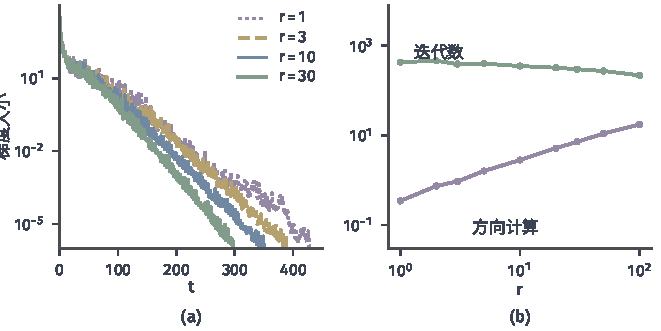
\includegraphics[width=112mm]{figures/05-optimization/02-smooth-optimization/matplotlib/qn-lbfgs-memory/figure.pdf}
  \caption{记忆长度的影响。目标是$200$维的$\sum_i(\tfrac12c_iz_i^2+\ln\cosh z_i)$，$\bm{z}=\bm{Q}\bm{x}$，$\bm{Q}$是固定的正交矩阵，$c_i$在$[10^{-3},10^{3}]$上对数等距，强Wolfe线搜索，$c_2=0.9$。(a)不同$r$下的梯度大小。(b)达到梯度大小$10^{-6}$的迭代数（绿）和这些迭代中方向计算的总乘法次数（紫，单位百万次，按每步$4rn$估算）。}
  \label{fig:qn-lbfgs-memory}
\end{BookInlineFigure}

\paragraph{初始缩放的影响}
图~\ref{fig:qn-lbfgs-scaling}比较有缩放~\eqref{eq:qn-lbfgs-gamma}和始终用$\gamma=1$的两种做法，记忆长度都是$r=10$，目标的曲率整体偏大。

没有缩放时，单位矩阵相对于真实曲率过大，方向过长，线搜索不得不反复收缩，$292$轮迭代共用了$5012$次函数和梯度计算。有缩放时只用$130$轮迭代和$268$次计算。这个对比说明，在大尺度问题上，第~\ref{sec:qn-secant}节“优先试单位步长”的策略依赖矩阵有正确的尺度。

\begin{BookInlineFigure}
  \centering
  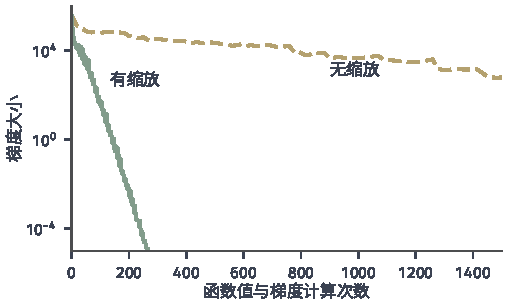
\includegraphics[width=86mm]{figures/05-optimization/02-smooth-optimization/matplotlib/qn-lbfgs-scaling/figure.pdf}
  \caption{初始缩放的影响：$r=10$，目标是$n=200$的旋转$\ln\cosh$函数（$c_i$在$[0.01,100]$上对数等距）再乘以$1000$，强Wolfe线搜索。绿线取式~\eqref{eq:qn-lbfgs-gamma}的缩放，黄虚线始终取$\gamma=1$。横轴是函数值与梯度的计算次数，纵轴是梯度大小。}
  \label{fig:qn-lbfgs-scaling}
\end{BookInlineFigure}
